\documentclass[12pt, oneside, a4paper, svgnames]{book}

\usepackage{array}
\usepackage[boxruled, linesnumbered]{algorithm2e}
\usepackage{amsmath}
\usepackage{amssymb}
\usepackage{amsthm}
\usepackage[toc]{appendix}
\usepackage{biblatex}
\usepackage{bm}
\usepackage{booktabs}
\usepackage{etoolbox}
\usepackage{fancyhdr}
\usepackage[a4paper, top=25.4mm, bottom=25.4mm, right=25.4mm,
left=40mm]{geometry}
\usepackage{graphicx}
\usepackage{hyperref}
\usepackage{istgame}
\usepackage{kbordermatrix}
\usepackage{listings}
\usepackage{mathtools}
\usepackage{minted}
\usepackage{multirow}
\usepackage[parfill]{parskip}
\usepackage{subcaption}
\usepackage{tikz}
\usepackage{xcolor}
 

\linespread{1.25}

\fancypagestyle{normal}{
	\fancyhf{}
	\fancyhead[L]{\slshape \leftmark}
	\fancyhead[R]{\thepage}
	\renewcommand{\headrulewidth}{0pt}
}

\fancypagestyle{chapterstyle}{
	\fancyhf{}
	\fancyhead[R]{\thepage}
	\renewcommand{\headrulewidth}{0pt}
}


\patchcmd{\chapter}{\thispagestyle{plain}}{\thispagestyle{chapterstyle}}{}{}



\renewcommand{\kbldelim}{(}
\renewcommand{\kbrdelim}{)}


\renewcommand\arraystretch{1.5}
\renewcommand{\tabcolsep}{0.5cm}

\graphicspath{{images/}}



\addbibresource{{tex/references/main.bib}}


\theoremstyle{definition}
\newtheorem{definition}{Definition}[section]

\newtheorem{theorem}{Theorem}[section]


\usetikzlibrary{snakes}
\usetikzlibrary{positioning}


\begin{document}

\newgeometry{a4paper, top=25.4mm, bottom=25.4mm, right=25.4mm, left=25.4mm}
\begin{titlepage}
	\begin{center}
		\vspace*{0.5cm}
		\includegraphics[width=5cm]{cardiff-uni-logo.jpg}

		\vspace{1cm}

		\huge
		An Empirical Study on the Folk Theorem

		\vspace{2cm}

		\large
		Student: Sophie Shapcott

		\vspace{0.5cm}

		Supervisor{(s)}: Dr Vince Knight and Henry Wilde 

		\vspace{0.5cm}

		Academic Year: 2019/20
		
		\vspace{0.5cm}

		School of Mathematics, \\Cardiff University

		\vfill

		\normalsize
		A final year undergraduate project submitted in partial fulfilment of the\\ requirements for MMORS (Masters in Mathematics, Operational Research\\ and Statistics) taught programme.

	\end{center}
\end{titlepage}

\restoregeometry

\frontmatter
\pagestyle{chapterstyle}
\chapter{Summary}

This project consists of an empirical study into a class of theorems, entitled
`Folk Theorems', which are a key part of the repeated games theory. The aims of
the project include: an in-depth review of academic literature regarding the
topic; the development and execution of a large experiment based on the
`original' folk theorem of Friedman~\cite{Friedman1971} with the Iterated
Prisoner's Dilemma; and an analysis of the effects of different tournament
characteristics on the \(p\)-threshold appearing in the folk theorems. These
ideas are extended from a third year assignment in Game Theory, completed by the
author.

Firstly, after an introduction to the theory of one-shot and repeated games, a
search of the folk theorem literature is provided in Chapter~\ref{ch:Lit_Review}. This reveals the vast
directions of research in the area for the past fifty years. Many
generalisations and refinements of the folk theorem have been analysed since the
first written papers in the 1970s. The games for which the notion has been
expanded to range from complete information games to games with imperfect
private monitoring. However, in certain cases, the strategies used in the proof
of these are unstable. Also, in situations where an individual deviator cannot
be identified, a much smaller set of payoffs can be achieved, yielding the
so-called `Anti-Folk Theorems'. More recently, focus has been on the application
of the folk theorem to computing and quantum transportation, for example.
Finally, it is concluded that, to the best of the author's knowledge, this is
the fist study to execute an experiment on the folk theorem of this size.

Following this, a detailed description of how the experiment was set-up and
executed is provided in Chapter~\ref{ch:Methods}, with justifications to the specific methods and software
chosen. After considering the benefits and drawbacks of varying file formats for
storing data, it is stated that a relational database, in particular SQLite,
would be the most appropriate. This is due to: the existence of libraries in
Python enabling the easier access of the data; the general robustness of
databases; and its ability to perform out of memory operations. Due to the
pre-existing game theoretic libraries, Axelrod and Nashpy, Python was chosen as
the language of implementation and ensuring good software development principles
were followed is highlighted as a priority. The volume of data which was planned
to be collected meant that remote computing was required and is explained in
this chapter. Here, the choice of support enumeration for the calculation of
Nash equilibria and the potential issues which may be faced due to degeneracy is
also discussed.

The main analysis of the data collected is provided in
Chapter~\ref{ch:Analyses}. An initial analysis discussing the characteristics of
the strategies used and the overall summary statistics is detailed, before the
\(p\)-thresholds are explored. The characteristics of tournaments focused on
are: the number of opponents the Defector had and the level of tournament noise
included. However, this is concluded as a non-trivial task due to the
uncertainty regarding the degeneracy of a large proportion of tournament sets.
Also, the inevitability of randomness within the tournaments meant that a lot
more data than what was obtained is required. On the other hand, the graphs that
were yielded are stated as successful in visualising the folk theorem.

Finally, Chapter~\ref{ch:Conclusions_and_Recommendations} details the
conclusions of the research before giving recommendations for further work.
Amongst these were suggestions on how more characteristics of the tournament set
could be studied as well as the potential to predict the \(p\)-threshold from
the characteristics of the tournaments via regression analysis.
\chapter{Acknowledgements}

First and foremost, I would like to express my sincere thanks and gratitude to
my project supervisors Dr Vince Knight and Henry Wilde for their continual
advice, support and invaluable ideas throughout the completion of this project.
You have always been willing to lend a hand or provide encouragement when
it was needed the most. I do not think I could have gotten better supervisors
and I apologise for not achieving everything in the plan. You have assisted me
through what will probably be the largest project I will ever do!

There are many people who have helped and supported me, both inside and outside
university, over the past four years of my undergraduate degree here at Cardiff
School of Mathematics. If I was to mention all the names, this would be longer
than my whole project! Therefore, this `thank you' is for all those who I have
had the pleasure of being taught by and working with during my degree. You have
made this journey an interesting and enjoyable one and I will continue to be
inspired by the passion all the lecturers have for what they do. 

Also, I would like to give special mention to Nikoleta, who, even though is in
her final few months of a PhD (probably the most challenging period), found time
to have chats with me and make sure I was still operating on this planet. You
encouraged me and always had a positive thing to say when I was convinced
everything was going to end terribly. So thank you very much Nikoleta, for being
such a great friend and best of luck with the completion of your thesis!

Last but most certainly not least, I want to say a huge thank you to my Mum, Dad
and Zoe for their continual love and support. To say these have been a
challenging four years is an understatement but you were always there for me
through it all. If it was not for your belief that I could achieve it I do not
think I could have completed this project, let alone the past four years! My
Mum, thank you for keeping me fuelled with coffee and biscuits through the long
days and for being a shoulder to cry on when necessary (I will pay you back with
hair dye, for all those grey ones I caused!). Dad, thank you for making me laugh
(and cry) with your terrible jokes and I promise I will replace all those grains
of coffee I had from `your' coffee pot. Finally, my sister Zoe (yes, you are
getting a mention because, yes, you did play a key part) thank you for keeping
me sane and always making me smile.

To all those who I have forgotten to mention: my sincerest apologies and thank
you for all your support.

\tableofcontents
\listoffigures

\mainmatter
\pagestyle{normal}

\chapter{Introduction}\label{ch:Introduction}

Game Theory is the study of interactive decision making and developing
strategies through mathematics~\cite{Dictionary2013}. It analyses and gives
methods for predicting the choices made by players (those making a decision),
whilst also suggesting ways to improve their `outcome'
~\cite{maschler_solan_zamir_2013}. Here, the abstract notion of utility is what
the players wish to maximise (see Chapter 2 in~\cite{maschler_solan_zamir_2013}
for a detailed discussion on the topic of utility theory or Section 1.3
~\cite{Webb2007} for a more introductory explanation). One of the earliest
pioneers of game theory is mathematician, John von Neumann who, along with
economist Oskar Morgenstern, published \textit{The Theory of Games and Economic
Behaviour} in 1944~\cite{maschler_solan_zamir_2013}. This book discusses the
theory, developed in 1928 and 1940-41, by von Neumann, regarding ``games of
strategy'' and its applications within the subject of economics
~\cite{von2007theory}. Following this, several advancements have been made in
the area, including, most notably, John Nash's papers on the consequently named
Nash Equilibria in 1950/51~\cite{nash1950equilibrium, nash1951non}. Due to the
``context-free mathematical toolbox''~\cite{maschler_solan_zamir_2013} nature of
this subject, it has been applied to many areas, from
networks~\cite{liang2012game, 1593279} to biology~\cite{chen2009robust, 
adeoye2012application}. In this project, the main focus is on a
particular class of theorems, within game theory, known as ``Folk Theorems''
with application to the game of A Prisoner's Dilemma. These will be defined and
discussed in the subsequent sections.

\section{An Introduction to Games}\label{sec:An_Intro_to_Games}
Consider the following scenario:

\begin{center}
    Two convicts have been accused of an illegal act. Each of these prisoners,
    separately, have to decide whether to reveal information (defect) or stay
    silent (cooperate). If they both cooperate then the convicts are given a
    short sentence whereas if they both defect then a medium sentence awaits.
    However, in the situation of one cooperation and one defection, the prisoner
    who cooperated has the consequence of a long term sentence, whilst the other
    is given a deal.~\cite{Knight2017}
\end{center}

This is one of the standard games in game theory known as A Prisoner's Dilemma.
It has four distinct outcomes, for the given two player version, which can be
represented as a table (see Table~\ref{tab:PD_outcomes}).
\begin{table}
\begin{tabular}{ cc|c|c|c| }\label{tab:PD_outcomes}
    \cline{3-4}
     & & \multicolumn{2}{ c| }{Column Player} \\
    \cline{3-4}
     & & coop & defect \\
    \multicolumn{1}{ |c }{\multirow{2}{*}{Row Player}} &
    \multicolumn{1}{ |c| }{coop} & (3, 3) & (0, 5) \\
    \cline{2-4}
    \multicolumn{1}{ |c }{} & 
    \multicolumn{1}{ |c| }{defect} & (5, 0) & (1, 1) \\
    \cline{1-4}
\end{tabular}
\caption{Outcomes \& payoffs for the game of A Prisoner's Dilemma.}\label{tab:PD_outcomes}
\end{table}
Each coordinate \((a, b)\) in the table represents the utility values obtained
for each player, where \(a\) is the utility value obtained by the row player
and \(b\) is the utility gained by the column player. These utility values are
as given in~\cite{axelrod1980effective} and are used throughout this project.
More formally, the game can be represented as the following matrix:

\kbordermatrix{
    \mbox{ } & coop & defect\\ 
    coop & (3, 3) & (0,5)\\ 
    defect & (5, 0) & (1, 1)
}\label{PDMatrix}

which is known as a \emph{normal form} representation of the game. The following
definition is adapted from~\cite{maschler_solan_zamir_2013}.

In general a \textit{normal form} or \textit{strategic form} game is defined by
an ordered triple \(G = (N, (S_i)_{i \in N}, (u_i)_{i \in N})\), where:
\begin{itemize}
    \item \(N = \{1, 2,\ldots, n\} \) is a finite set of players;
    \item \(S = S_1 \times S_2, \times \cdots \times S_n\) is the set of
    strategies for all players in which each vector \((S_i)_{i \in N}\) is the
    set of strategies for player i~\footnote{Since the game of A Prisoner's
    Dilemma has a finite strategy set for each player \(S_i = \{
    \text{cooperate}, \text{defect}\} (i \in N)\), in this project only finite
    strategy spaces are considered.}; and
    \item \(u_i : S \to \mathbb{R}\) is a payoff function which associates each
    strategy vector, \(\textbf{s} = (s_i)_{i \in N}\), with a utility~\footnote{'Utility' is referred to as a player's `payoff' throughout the
    remainder of this report.} \(u_i(i \in N)\).
\end{itemize}

Yet another way of representing this game is as a pair of matrices, \(A, B\),
defined as follows:
\[
    A = 
    \begin{pmatrix}
       3 & 0\\
       5 & 1\\ 
    \end{pmatrix}
    \text{ and } B = A^{T} =
    \begin{pmatrix}
        3 & 5\\
        0 & 1\\
    \end{pmatrix}
\]
This way of defining games allow for the use of calculating payoffs for each
player (see Section~\ref{sec:NE_for_Normal_Form_Games}).

Before continuing the discussion into the key notions of game theory, it needs
to be highlighted that there is an important assumption, which is central to
most studies of game theory, entitled \textit{Common Knowledge of Rationality}.
This, more formally, is an infinite list of statements which claim:
    \begin{itemize}
        \item The players are rational;
        \item All players know that the other players are rational;
        \item All players know that the other players know that they are 
        rational; etc.    
    \end{itemize}
Assuming Common Knowledge of Rationality allows for the prediction of rational
behaviour through a processes entitled \textit{rationalisation}
~\cite{Knight2019}
(see section 4.5 in~\cite{maschler_solan_zamir_2013} for an alternative
explanation of this assumption). 


A strategy for player \(i\), \(s_{i}\), is \textit{strictly dominated} if there
exists another strategy for player \(i\), say \(\bar{s_{i}}\), such that for all
strategy vectors \(s_{-i} \in S_{-i}\) of the other players, 
\[
    u_{i}(s_{i}, s_{-i}) < u_{i}(\bar{s_{i}}, s_{i}).
\]
In this case we say that \(s_{i}\) is \textit{strictly dominated} by
\(\bar{s_{i}}\). Here, 
\(s_{-i} = \{s_{1}, s_{2}, \ldots, s_{i-1}, s_{i+1}, \ldots, s_{n}\} \), i.e. \
the \(i\)th player's strategy has been omitted. The 
set, \(S_{-i}\), is defined similarly. Looking at the row player's matrix of a
Prisoner's Dilemma~\ref{PDMatrix} (the first entries in the ordered tuples), it
is clear that cooperation is a strictly dominated strategy. Due to the
symmetricity of the game, this is also true for the column
player.~\cite{maschler_solan_zamir_2013}



So far, only the pure strategies, \(S_{i}=\{\text{coop}, \text{defect}\} \), have
been discussed, thus the notion of a probability distribution over \(S_{i}\) is
now introduced, giving the so-called \textit{mixed strategies} as defined in~\cite{maschler_solan_zamir_2013}:
Let \(G=(N, (S_{i})_{i \in N}, (u_{i})_{i \in N})\) be a game (with each 
\(S_{i}\) finite), then a \textit{mixed strategy} for player \(i\) is a
probability distribution over their strategy set \(S_{i}\). Define:
\[
\Sigma_{i} := \{\sigma_{i} : S_{i} \to [0, 1] : \sum_{s_{i} \in S_{i}}{\sigma_
{i}(s_{i})} = 1\}   
\]
to be the set of mixed strategies for player \(i\). Hence, observe that the pure
strategies are specific cases of mixed strategies, with \(\sigma_{i} = (1, 0)\)
for cooperation and \(\sigma_{i} = (0, 1)\) for defection, in the example of a
Prisoner's Dilemma.

This leads onto the following definition of a \emph{mixed extension} of a game,
taken from~\cite{maschler_solan_zamir_2013}:
Let \(G\) be a finite normal form game as above, with \(S = S_{1} \times
S_{2} \times \cdots \times S_{N}\) defining the pure strategy vector set and
each pure strategy set, \(S_{i}\) being non-empty and finite. Then the
\textit{mixed extension} of \(G\) is denoted by
\[
    \Gamma = (N, (\Sigma_{i})_{i \in N}, (U_{i})_{i \in N}),
\]
and is the game in which, \(\Sigma_{i}\) is the \(i\)th player's strategy set
and \(U_{i} : \Sigma \to \mathbb{R}\) is the corresponding payoff function,
where each \(\sigma = (\sigma_{1}, \sigma_{2}, \ldots, \sigma_{N}) \in \Sigma =
\Sigma_{1} \times \Sigma_{2} \times \cdots \times \Sigma_{N}\) is mapped to the
payoff
\begin{equation}
    U_{i} = \mathbb{E}_{\sigma}(u_{i}(\sigma)) = \sum_{(s_{1}, s_{2}, \ldots, s_
    {N}) \in S}{u_{i}(s_{1}, s_{2}, \ldots, s_{N})\sigma_{1}(s_{1})\sigma_{2}(s_
    {2})\cdots\sigma_{N}(s_{n})} 
\end{equation}\label{eqn:mixed_payoff_function}
for all players \(i \in N\).

\section{Nash Equilibrium for Normal Form Games}\label{sec:NE_for_Normal_Form_Games}
As mentioned above, mathematician, John Nash, introduced the concept of an
equilibrium point and proved the existence of mixed strategy Nash Equilibria in
all finite games. These notions are central to the study of game
theory~\cite{maschler_solan_zamir_2013} and hence, in this section, Nash's
concepts will be defined and proved in detail.

Firstly, before the definition of a Nash equilibrium, the idea, as given 
in~\cite{maschler_solan_zamir_2013} of a \textit{best response} is introduced:
For a game \(G=(N, (S_{i})_{i \in N}, (u_{i})_{i \in N})\), the strategy,
\(s_{i}\), of the \(i\)th player is considered a \textit{best response} to the
strategy vector \(s_{-i}\) if \(u_{i}(s_{i}, s_{-i}) = \max_{t_{i} \in
S_{i}}u_{i}(t_{i}, s_{-i})\).

This leads onto the main definition of the section:
\begin{definition}\label{def:NE}
    Given a game \(G=(N, (S_{i})_{i \in N}, (u_{i})_{i \in N})\), the vector of
    strategies \(s^{*} = (s_{1}^{*}, s_{2}^{*}, \ldots, s_{n}^{*})\) is a
    \textit{Nash equilibrium} if, for all players \(i \in N\), \(s_{i}^{*}\) is 
    a best response to \(s_{i}^{*} \in N\).~\cite{maschler_solan_zamir_2013}
\end{definition}
In other words, \(s^{*}\) is a Nash equilibrium if and only if no player has any
reason to deviate from their current strategy \(s_{i}^{*}\).

Recall that, in Section~\ref{sec:An_Intro_to_Games}, for any player in A
Prisoner's Dilemma, defection dominated cooperation. This leads to the following
observation:
\begin{center}
    \textbf{The strategy pair (Defect, Defect), is the unique Nash equilibrium 
    for A Prisoner's Dilemma, with a payoff value of 1 for each player.}~\cite{maschler_solan_zamir_2013}
\end{center}
This can be visualised as followed:
Assume the row player uses the following mixed strategy, \(\sigma_{r} = (x,
1-x)\), i.e. \ the probability of cooperating is \(x\) and the probability of
defecting is \(1-x\). Similarly, assume the column player has 
the strategy, \(\sigma_{c} = (y, 1-y)\). The payoff obtained for the row and column player, respectively, is then:
\[
    A\sigma_{c}^T = \begin{pmatrix}
        3 & 0 \\
        5 & 1
    \end{pmatrix} \begin{pmatrix}
        y \\
        1-y
    \end{pmatrix} = \begin{pmatrix}
        3y \\
        4y + 1
    \end{pmatrix},
\]
\[
    \sigma_{r}B = \begin{pmatrix}
        x & 1-x
    \end{pmatrix} \begin{pmatrix}
        3 & 5 \\
        0 & 1        
    \end{pmatrix}  = \begin{pmatrix}
        3x & 4x + 1
    \end{pmatrix}
\]

Plotting these gives the following:
\begin{figure}[h]
    \centering
        \begin{subfigure}[t]{0.45\textwidth}
        \centering
            \includegraphics[width=\linewidth]{{pd-row-payoff}}
        \end{subfigure}
    \hfill
        \begin{subfigure}[t]{0.45\textwidth}
        \centering
            \includegraphics[width=\linewidth]{{pd-col-payoff}}
        \end{subfigure}~\caption{Graphs to show the row and column players' payoffs against a 
        mixed strategy.}\label{fig:mixed_strategy_PD}
    \end{figure}
From Figure~\ref{fig:mixed_strategy_PD} it is clear that, regardless of the
strategy played by the opponent, defection is indeed the only rational move for
one to play. Thus, both players have no incentive to deviate if and only if both
play the strategy \(\sigma=(0, 1)\), i.e. \ defection for every single game of A
Prisoner's Dilemma.

On the other hand, consider, for example, a game with no dominated
strategies~\footnote{The game highlighted here is another standard used in game
theory entitled \emph{Matching Pennies}. Moreover, it is what is defined as a
\emph{zero-sum} game. Interested readers are encouraged to read Example 4.21
of~\cite{Webb2007} for an introduction to the game and Section 4.12
in~\cite{maschler_solan_zamir_2013} for an explanation of zero-sum games.}:
\[
    A =
    \begin{pmatrix}
        1 & -1\\
        -1 & 1\\
    \end{pmatrix}, \ B =
    \begin{pmatrix}
        -1 & 1\\
        1 & -1\\
    \end{pmatrix}
\]
Are Nash Equilibria guaranteed to exist? This result is given in the next
theorem, taken from~\cite{nash1951non}, Nash's second paper on equilibria in 
games.

\begin{theorem}\label{thm:Nash}
    Every finite game has an equilibrium point.
\end{theorem}

The proof of Theorem~\label{thm:Nash} includes the use of a \emph{fixed point
theorem} and thus, a short sub-section regarding one such result is given, for
completeness, before providing a formal proof of~\ref{thm:Nash}.

\subsection{Brouwer's Fixed Point Theorem}\label{subsec:Brouwer_thm}
Brouwer's Fixed Point Theorem is a result from the theory of topology. Named
after the Dutch mathematician, L.E.J. Brouwer, it was proven in
1912~\cite{Carlson2016}. However, before stating this notion, a few conditions
regarding the properties of sets are recalled. 

The following three definitions appear as 
in~\cite{Weisstein, Barile, Weissteina} respectively:
\begin{definition}
    A set \(X \subseteq \mathbb{R}^{d}\) is called \textit{convex} if it
    contains all line segments connecting any two points \(\textbf{x}_{1},
    \textbf{x}_{2} \in X\).
\end{definition}

\begin{definition}
    An \textit{open cover} of a set \(S \subset X\), a topological space, is a
    collection of open sets \(A_{1}, A_{2}, \ldots \subset X\) such that
    \(A_{1} \cup A_{2} \cup \ldots \supset S\), that is, the union of the open
    sets contain S.
\end{definition}

\begin{definition}
    A subset \(S \subseteq X\), a topological space, is called \textit{compact}
    if, for each open cover of \(S\), there is a finite sub-cover of S.
\end{definition}

The presentation of Brouwer's Fixed Point Theorem is now given as 
in~\cite{maschler_solan_zamir_2013}
\begin{theorem}\label{thm:Brouwer}
    Let \(X \subseteq \mathbb{R}^{n}\) be a non-empty convex and compact
    set, then each continuous function \(f : X \to X\) has a fixed point.  
\end{theorem}
In other words if \(X\) and \(f\) satisfy the conditions given above then there
exists a point \(x \in X\) such that \(f(x) = x\). 

Since this project is regarding game theory, rather than topology, the proof to
the above theorem is omitted. However, the interested reader is referred
to~\cite{} for an in-depth consideration into the theory of topology.

\subsection{Proof of Nash's Theorem (Theorem~\ref{thm:Nash})}\label{subsec:Nash_Proof}
The proof provided here is adapted from the original, by Nash, as presented
in~\cite{nash1951non} (with extra notes adapted 
from~\cite{maschler_solan_zamir_2013}). According
to~\cite{maschler_solan_zamir_2013}, the general idea here is to define a
function, which satisfies the conditions required for Theorem~\ref{thm:Brouwer},
using the payoff functions on the set of mixed strategies. Then by identifying
each equilibrium point with a fixed point of the function, the required result 
is obtained.

\begin{proof}
    Firstly, a brief restatement of the notation needed is provided for clarity.
    Let \(G=(N, (S_{i})_{i \in N}, (u_{i})_{i \in N})\) be a finite game with
    mixed extension \(\Gamma=(N, (\Sigma_{i})_{i \in N}, (U_{i})_{i \in N})\).
    Here, \(N\) denotes the number of players; \(S = S_{1} \times S_{2} \times
    \ldots \times S_{N}\) is the set of pure strategies for all players, with
    \((S_i)_{i \in N}\) the pure strategy set for player i; \(\Sigma \) is
    defined similarly but relating to mixed strategies; and \(U_{i}: \Sigma \to
    \mathbb{R}\) are the payoff functions as given in
    equation~\ref{eqn:mixed_payoff_function}. Recall that \(\sigma_{-i}\) is
    used to denote the strategy choice of all players \emph{except} the \(i\)th
    player.
    
    Let \(\sigma = (\sigma_{1}, \sigma_{2}, \ldots, \sigma_{N})\) be a tuple of
    mixed strategies and \(U_{i,t}(\sigma)\) be the \(i\)th player's payoff if
    they changed to their \(t\)th pure strategy and all other players continue
    to use their mixed strategy.
    Now, define function \(f: \Sigma \to [0, \infty)\) such that 
    \begin{equation}
        f_{i,t}(\sigma) = \max{(0, U_{i,t}(\sigma)-U_{i}(\sigma))}
    \end{equation}
    and also let 
    \begin{equation}
        \sigma_{i}^{\prime} = \frac{ \sigma_{i}+\sum_{t}{f_{i,t}(\sigma)s_{i}^{t}} }{ 1+\sum_{t}{f_{i,t}(\sigma)} }
    \end{equation}
    be a modification of each \(\sigma_{i} \in \sigma \), with \(\sigma^{\prime}
    = (\sigma_{1}^{\prime}, \sigma_{2}^{\prime}, \ldots, \sigma_{N}^{\prime})\).
    In words, this modification increases the proportion of the pure strategy
    \(t\) used in \(\sigma_{i}\) if the payoff gained by the \(i\)th player is
    larger when they replace their mixed strategy by \(t\). Else, it remains the
    same if doing this decreases their payoff as \(f_{i,t}(\sigma)=0\) in this
    case. Note, the denominator ensures that the ending vector is still a
    probability distribution by standardising.

    The aim is to apply Theorem~\ref{thm:Brouwer} to the mapping \(T: \sigma \to
    \sigma^{\prime}\) and show that it's fixed points correspond to Nash
    equilibria. Thus, firstly compactness and convexity of the set \(\sigma \)
    is shown along with continuity of the function \(f\). 
    
    Observe that each \(\sigma_{i}\) can be represented by a point in a simplex
    in a real vector space with the vertices given by the pure strategies,
    \(s_{i}^{t}\). Therefore, it follows that the set \(\Sigma_{i}\) is convex
    and compact. Using the result, \textit{If \(A \subseteq \mathbb{R}^{n}\) and
    \(B \subseteq \mathbb{R}^{m}\) are convex compact sets then the set \(A
    \times B\) is a convex compact subset of \(\mathbb{R}^{n+m}\)}, as
    highlighted in~\cite{maschler_solan_zamir_2013} gives the convexity and
    compactness of the set \(\Sigma \), the cross product of all
    \(\Sigma_{i}\)s. 
    
    The continuity of the function \(f\) depends upon the continuity of the
    payoff functions \(U_{i}\). As given in~\cite{maschler_solan_zamir_2013},
    this is shown by first proving that the \(U_{i}\) are multilinear functions
    in the variables \((\sigma_{i})_{i \in N}\) and then applying the fact that
    any multilinear function over \(\Sigma \) is a continuous
    function.~\footnote{For a detailed consideration of the continuity of the
    payoff functions, please see~\cite{maschler_solan_zamir_2013}, pages
    148-149.} The result then follows.

    Hence, by Theorem~\ref{thm:Brouwer}, the mapping \(T\) must have at least
    one fixed point. The proof is concluded by showing that any fixed points of
    \(T\) are Nash equilibria. 

    Suppose \(\sigma \) is such that \(T(\sigma) = \sigma \). Then, the
    proportion of \(s_{i}^{t}\) used in the mixed strategy \(\sigma_{i}\) must
    not be altered by \(T\). Therefore, in \(\sigma_{i}^{\prime}\), the sum
    \(\sum_{t}{f_{i,t}(\sigma)}\), in the denominator, must equal zero.
    Otherwise, the total sum of the denominator will be greater than one,
    decreasing the proportion of \(s_{i}^{t}\). This implies that for all pure
    strategies \(q\), \(f_{i,q}(\sigma)=0\). That is, player \(i\) can not
    improve their payoff by adopting any of the pure strategies. Note, this is
    true for all \(i\) and \(q\) by definition of \(T(\sigma) = \sigma \) and
    thus no player is able to improve their payoff. By definition~\ref{def:NE},
    this is exactly the conditions of a Nash equilibrium.

    Now assume \(\sigma \) is a Nash equilibrium. Then, by definition, it must
    be that \(f_{i,q}(\sigma)=0\) for all pure strategies \(q\) for all players,
    \(i \in N\). Note, if \(f_{i,q}(\sigma) \ne 0\), then the
    \(i\)th player would benefit from changing their strategy to the pure
    strategy \(q\), which violates the condition for a Nash equilibrium. From
    this it follows that \(T(\sigma) = \sigma \), that is, \(\sigma \) is a
    fixed point of \(T\). This concludes the proof.

\end{proof}

\section{Repeated Games}\label{sec:Repeated_Games}
The folk theorems studied in this project are a consequence of games which are
repeated several times (not just once). Thus, before discussing the main ideas,
the theory of both finitely- and infinitely- repeated games is presented.

Firstly, a couple of alterations to the terminology used in
previous sections is redefined for conciseness and to be consistent with the
literature~\cite{}. What was known as a `game' will become known as a
\emph{stage game} to highlight the fact that a one-off game is being considered.
Also, what was defined previously as a `strategy' will now be referred to as an
\emph{action} to differentiate it from a strategy of a repeated game (see
Section~\ref{subsec:Finite_Repeated_Games}).

\subsection{Finite Repeated Games}\label{subsec:Finite_Repeated_Games}
According to~\cite{Knight2017a}, a \textit{\(T\)-stage repeated game}, \(T <
\infty\) is when the stage game, \(G\), is played \(T\) times, over discrete
time intervals. Each \(i\)th player has a strategy based on previous `rounds' of
the game and the payoff of a repeated game is calculated as the total sum of the
stage game payoffs.

Prior to giving the notion of a strategy in a repeated game, the idea of 
\emph{history}, within the context of repeated games, is provided.
The \textit{history}, \(H(t)\) of a repeated game is the knowledge of previous
actions of all players up until the \(t\)th stage game, assumed to be known by
player \(i\) for all \(i \in 1, \ldots, N\). Note that, when \(t=0\), \(H(0) =
\underbrace{(\emptyset, \emptyset, \ldots, \emptyset)}_{N \text{times}}\), since
no stage games have yet been played.

As given in~\cite{Knight2019a}, a \textit{strategy} of a \(T\)-stage repeated
game is defined to be a mapping from the complete history so far to an action of
the stage game, that is 
\[
    \tau_{i} : \cup_{t = 0}^{T-1}{H{t}} \to a_{i}. 
\]
Here, \(H(t)\) is the history of play as defined above and \(a_{i}\) is the
\(i\)th player's action of the stage game. 

Consider, for example, the environment in which the stage game of a Prisoner's
Dilemma is repeated each time. This is known as the \emph{Iterated Prisoner's
Dilemma} (IPD) and has been a popular topic of research for many years see
Chapter~\ref{ch:Literature_Search}. Note that the ojective here is to maximise
your payoff. The player: 
\begin{center}
    \textit{No matter what my opponents play, I will always defect},
\end{center}
commonly known as the `Defector' has the following strategy mapping:
\[
    \tau_{i} : \cup_{t = 0}^{T-1}{H{t}} \to a_{i},
\]
where \(a_{i}=D\) for all time periods \(\tau \ge 0\). Other common IPD
strategies include: 
\begin{center}
    Cooperator - \textit{No matter what my opponents play, I will always
    cooperate};
    Random - \textit{I will either cooperate or defect with a probability of
    50\%}; and
    \newline Tit For Tat - \textit{I will start by cooperating but then will 
    duplicate the most recent decision of my opponent.}
\end{center}

Figure~\ref{fig:2-stage_payoff_plot} shows the possible payoffs obtained in a 
2-stage repeated IPD with two players:

\begin{figure}
    \begin{tikzpicture}[scale=0.5]
        \draw (0, 0) -- (11, 0);
        \draw (0, 0) -- (0, 11);
        \foreach \x in {0,1,2,3,4,5,6,7,8,9,10,11}
            \draw (\x cm,1pt) -- (\x cm,-1pt) node[anchor=north] {$\x$};
        \foreach \y in {0,1,2,3,4,5,6,7,8,9,10,11}
            \draw (1pt,\y cm) -- (-1pt,\y cm) node[anchor=east] {$\y$};
        \filldraw [blue] (2, 2) circle (2pt);
        \filldraw [blue] (0, 10) circle (2pt);
        \filldraw [blue] (10, 0) circle (2pt);
        \filldraw [blue] (6, 6) circle (2pt);
        \filldraw [blue] (3, 8) circle (2pt);
        \filldraw [blue] (8, 3) circle (2pt);
        \filldraw [blue] (1, 6) circle (2pt);
        \filldraw [blue] (6, 1) circle (2pt);
        \filldraw [blue] (4, 4) circle (2pt);
    \end{tikzpicture} 
    \caption{A plot to show the possible payoffs of the game between two players in which A Prisoner's Dilemma is repeated twice.}\label{fig:2-stage_payoff_plot}
\end{figure}


Now, what about Theorem~\ref{thm:Nash}? Are there any Nash equilibria in
repeated games? In fact, it can be proven that there exist many equilibria
in repeated games~\cite{friedman1971non}. The next result, adapted
from~\cite{Knight2019a} guarantees at least one Nash equilibria.
\begin{theorem}\label{thm:seq_of_stage_NE}
    Consider a \(T\)-stage repeated game with \(G=(N, (S_{i})_{i \in N},
    (u_{i})_{i \in N})\) as the stage game, \(0 < T < \infty \). Define by
    \(\bm{\sigma}^{*} =(\sigma_{1}^{*}, \sigma_{2}^{*}, \ldots, \sigma_{N}^{*})\),
    a stage Nash equilibrium of \(G\). Then the sequence in which
    \(\bm{\sigma}^{*}\) is continuously played is a Nash equilibrium of the
    \(T\)-stage repeated game.
\end{theorem} 

\begin{proof}
    Since \( \bm{\sigma}^{*} \) is a stage Nash equilibrium, it is, in particular,
    a Nash equilibrium of the \(T\)th stage game. Thus, no player has any reason
    to deviate here. But then \( \bm{\sigma}^{*} \) was also played at the
    \((T-1)\)th stage also, meaning there is still no reason to deviate.
    Therefore, continuing via backwards induction gives the required result.
\end{proof}

Hence, for the \(T\)-stage IPD, every player executing the Defector strategy
yields a Nash equilibrium. However, do there exist equilibria for which
selecting the action `cooperate' is more beneficial?

In preparation to answer this, the next
Subsection~\ref{subsec:Infinite_Repeated_Games} discusses the case when \(T \to
\infty \) and results linked to \emph{infinitely repeated games}.

\subsection{Infinite Repeated Games}\label{subsec:Infinite_Repeated_Games}
The Folk Theorem discussed in Section~\ref{sec:Folk_Thm} considers a stronger
notion of equilibria known as \textit{subgame perfect equilibria}. In order to
fully understand this notion, a new representation of games is introduced.

\subsubsection{Extensive Form Games}\label{subsubsec:Extensive_Form_Games}
According to~\cite{maschler_solan_zamir_2013}, an \textit{extensive form game}
is given by the ordered vector
\(\Gamma = (N, V, E, x_{0}, (V_{i})_{i \in N}, O, u)\)
where \(N\) is a finite set of players; \((V, E, x_{0})\) is a \textit{game
tree}~\footnote{The triple \((V, E, x_{0})\) is defined as a \textit{tree} if
the set of vertices, \(V\), and the set of edges, \(E\), create a
\textit{directed graph} (that is, each element in \(E\) is an ordered tuple) and
x_{0} represents the root, or starting node, of the graph.}; \((V_{i})_{i \in
N}\) is a partition of the set \(V \setminus L\), where \(L\) is the set of all
leaves, or terminal points, of the game tree; \(O\) is the set of outcomes for
the game; and \(u\) is a function which maps each leaf in \(L\) to an outcome 
in \(O\).

This leads on to the following definition, adapted from~\cite{Webb2007}:
\newline
A player's \textit{information set} is a subset of the nodes in a game tree
where:
\begin{itemize}
    \item Only the player concerned is deciding;
    \item This player is not aware of which node has been reached except that it
    is definitely one of the elements found in this set.
\end{itemize} 

In Figure~\ref{fig:PD_game_tree}, the extensive form representation of the
game A Prisoner's Dilemma is provided. Here, only two players are considered and
any information sets are represented by a dashed line. Note, any normal form
game can be represented as an extensive form game. 

\begin{figure}
    \begin{istgame}[scale=0.5]
    \setistgrowdirection'{east}
    \istroot(0){Player 1}
        \istb{coop}[a]
        \istb{defect}[b]
    \istroot(1)(0-1)
        \istb{coop}[a]{(3, 3)}
        \istb{defect}[b]{(0, 5)}
    \istroot(2)(0-2)
        \istb{coop}[a]{(5, 0)}
        \istb{defect}[b]{1, 1}
    \xtInfoset(1)(2){Player 2}     
    \end{istgame}
    \caption{The extensive form representation of A Prisoner's Dilemma.}\label{fig:PD_game_tree}
\end{figure}

According to~\cite{Webb2007}, a \textit{subgame} is a sub-graph of the game tree
such that:
\begin{itemize}
    \item The sub-graph begins at a decision node, say \(x_{i}\);
    \item This node, \(x_{i}\), is the only element contained in its information set;
    \item The sub-graph contains all of the decision nodes which follow \(x_{i}\).
\end{itemize}

This leads to the following definition of \emph{subgame perfect equilibria},
adapted from~\cite{Webb2007}.
\begin{definition}
    A \textit{subgame perfect equilibrium} is a Nash equilibrium which satisfies
    the condition that the strategies played define a Nash equilibrium in every
    subgame.
\end{definition}
Hence the strategy defined in Theorem~\ref{thm:seq_of_stage_NE} is a subgame
perfect equilibrium. A few final definitions are now highlighted before
introducing the Folk Theorem.

\subsubsection{Final Definitions Needed}\label{subsubsec:Final_Defs_Needed}
Now, in order to be able to discuss the payoffs of strategies in infinite games;
the notion of a \emph{discounted payoff} is introduced. This is defined
in~\cite{Knight2017b} as:
\[
    V_{i}(\sigma) = \sum_{t=1}^{\infty}{\delta^{t-1}U_{i}(\sigma)},
\]
where the discount factor, \(\delta \), can be thought of as the probability
that the game continues. That is, the probability that another stage game will
be played. Using this, the \textit{average payoffs}, per stage game, can be defined by:
\[
    \frac{1}{\bar{T}}V_{i}(\sigma) = (1-\delta)V_{i}(\sigma),
\]
where \(\bar{T} = \frac{1}{1-\delta}\) is the average length of a game
~\cite{Knight2017b}.

Finally, Figure~\ref{fig:Feasible_Payoff_Plot} shows those payoffs which are
individually rational for a two player version of A Prisoner's Dilemma. In
general, an \textit{individually rational payoff} is an average payoff which
exceeds the payoffs obtained in the stage Nash equilibria for all
players~\cite{Knight2017b}. Note, often the Nash equilibrium payoffs are not the
optimal payoff which players could achieve.

\begin{figure}
    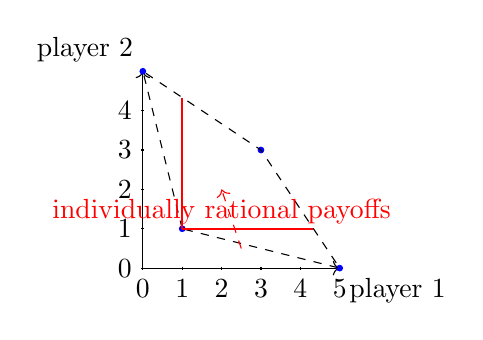
\begin{tikzpicture}[scale=0.5]
        \draw[->] (0,0) -- (5,0) node[anchor=north west] {player 1};
        \draw[->] (0,0) -- (0,5) node[anchor=south east] {player 2};
        \foreach \x/\xtext in {0,1,2,3,4,5}
            \draw (\x cm,1pt) -- (\x cm,-1pt) node[anchor=north] {$\xtext$};
        \foreach \y/\ytext in {0,1,2,3,4}
            \draw (1pt,\y cm) -- (-1pt,\y cm) node[anchor=east] {$\ytext$};
        \filldraw [blue] (1, 1) circle (2pt);
        \filldraw [blue] (0, 5) circle (2pt);
        \filldraw [blue] (5, 0) circle (2pt);
        \filldraw [blue] (3, 3) circle (2pt);
        \draw[black, dashed] (1,1) -- (0,5) -- (3,3) -- (5,0) -- (1,1);
        \draw[red, thick] (1, 1) -- (1, 13/3);
        \draw[red, thick] (1, 1) -- (13/3, 1);
        \draw[red, dashed, ->] (2.5, 0.5) -- (2, 2) node[anchor=north]{individually rational payoffs};
    \end{tikzpicture}
    \caption{A plot highlighting the possible individually rational payoffs for the game of A Prisoner's Dilemma.}\label{fig:Feasible_Payoff_Plot}
\end{figure}

In the next section (Section~\ref{sec:Folk_Thm}), the main theorem of this
project will be stated and proved.

\section{Folk Theorem}\label{sec:Folk_Thm}
According to~\cite{Webb2007}, the class of theorems known as Folk Theorems are
so-called because the result was well-known before a formal proof was provided.
In general, these theorems state that players can achieve a better payoff than
the Nash equilibrium (if the Nash equilibrium payoff is not optimal) when the
stage game is repeated many times and the probability of the game continuing is 
large enough. 

It is believed that Friedman, 1971 (~\cite{friedman1971non}) was one of the
first to publish a formal proof to the widely accepted Folk Theorem~\cite{}.
Thus, the presentation of the statement and proof given here is adapted
from~\cite{friedman1971non} as well as from~\cite{Knight2017b}.

Before stating the theorem, the list of assumptions which
Friedman~\cite{friedman1971non} requires the infinite repeated game to satisfy is given.
\begin{enumerate}
    \item The mixed action sets, \(\Sigma_{i}\) are compact and convex for all
    \(i\in N\). 
    \item The payoff functions, \(U_{i}: \Sigma \to \mathbb{R}\), are continuous
    and bounded for all \(i\in N\).
    \item The \(U_{i}(\sigma)\)s are quasi-concave~\footnote{According
    to~\cite{Stover}, a real-valued function \(f\), defined on a convex subset
    \(C \subset \mathbb{R}^n\), is \textit{quasi-concave} if for all \(\alpha
    \in \mathbb{R}\), the set \( \{ x \in C : f(x) \ge a \} \) is convex.}
    functions of \(sigma_{i}\) for all \(i\in N\).
    \item If  \(U_{i}^{\prime} \le U_{i}^{\prime\prime}\), for all \(i\in N\)
    and \(U_{i}^{\prime}, U_{i}^{\prime\prime} \in H\), then, for all
    \(U_{i}^{\prime} \le U \le U_{i}^{\prime\prime}\), \(U \in H\). Here, \(H\)
    is defined to be the set of feasible payoffs, \( \{ U(\sigma) : \sigma \in
    \Sigma \} \), where \(U(\sigma) = (U_{1}(\sigma), U_{2}(\sigma), \ldots,
    U_{N}(\sigma))\).
    \item  \(H^{*}\) is concave, where \(H^{*} \subset H\) denotes the set of
    all Pareto optimal payoffs.~\footnote{Friedman defines a \textit{Pareto
    optimal payoff} as a point in the payoff space \(U_(\sigma^{*})\) which
    satisfies the conditions: \(\sigma^{*} \in \Sigma \) and \(U_{i}(\sigma^{*})
    > U_{i}(\sigma)\) for all \(i \in N\)}.
    \item All stage games are identical in the infinitely repeated game.
    \item The discount parameter, \(\delta \), is equal in all time periods.
    \item The stage game has a unique Nash equilibrium.
    \item The Nash equilibrium is not Pareto optimal. 
\end{enumerate}
Note, Friedman~\cite{friedman1971non} later goes on to prove that assumptions
six to nine can be removed with only a small effect on the result. However,
since the only game being studied in this project is the IPD (which satisfies
all the above assumptions), this generalisation will be omitted. Thus, only the
proof of the original theorem will be provided.

\begin{theorem}\label{thm:Folk}
    If the above assumptions are all satisfied for the given infinite repeated
    game, then for any individually rational payoff \(V_{i}\) (greater than the
    payoff yielded by the stage Nash equilibrium \(\sigma^{ne}\)), there exists
    a discount parameter \(\delta^{*}\) such that for all \(\delta_{i}\), \(0 <
    \delta^{*} < \delta_{i} < 1\) there is a subgame perfect Nash equilibria
    with payoffs equal to \(V_{i}\).
\end{theorem}

\begin{proof}
    Consider the set of all actions which yield greater payoffs than the Nash
    equilibrium, denoted by:
    \[
        B = \{\sigma : \sigma \in \Sigma, U_{i}(\sigma) > U_{i}(\sigma^{ne}), i = 1, 2, \ldots, N\}
    \]
    and define the following trigger strategy:
    \begin{equation}
        \sigma_{i1} = \sigma_{i}^{\prime}, \newline
        \sigma_{it} = \begin{cases}
            \sigma_{i}^{\prime}, & \quad \text{if } \sigma_{j\tau}=\sigma_{j}^{\prime} \ j \ne i, \tau=1, 2, \ldots, t-1, t=2, 3, \ldots \\
            \sigma_{i}^{ne}, & \quad \text{otherwise},
        \end{cases}
    \end{equation}\label{eqn:trigger_strategy}
    where \(\sigma_{i}^{\prime} \in B\). In words, the \(i\)th player will choose \(\sigma_{i}^{\prime}\) unless any
    other player does not play \( \sigma_{j}^{\prime}\), in which case they
    continue by playing their Nash equilibrium action, \(\sigma_{i}^{ne}\). Now,
    by definition, the strategy in~\ref{eqn:trigger_strategy} is an equilibrium
    of the repeated game if 
    \[
        \sum_{\tau=0}^{\infty}{\delta_{i}^{\tau}U_{i}(\sigma_{i}^{\prime})} > U_{i}(\sigma_{-i}^{\prime}, t_{i}) + \sum_{\tau=1}^{\infty}{\delta_{i}^{\tau}U_{i}(\sigma^{ne})}, \ \ i=1, 2, \ldots, N,
    \]
    which can be rearranged to 
    \[
        \frac{\delta_{i}}{1-\delta_{i}}[U_{i}(\sigma^{\prime}) - U_{i}(\sigma^{ne})] > U_{i}(\sigma_{-i}^{\prime}, t_{i}) - U_{i}(\sigma{\prime}), \ \ i=1, 2, \ldots, N,
    \]
    where \(U_{i}(\sigma_{-i}^{\prime}, t_{i}) = \max_{\sigma_{i} \in
    \Sigma_{i}}{U_{i}(\sigma_{-i}^{\prime}, \sigma_{i})}\), \(t_{i} \in
    \Sigma_{i}\).

    To check if this strategy is indeed a best response to all others players,
    who are executing the same strategy in~\ref{eqn:trigger_strategy}, for the
    \(i\)th player consider their alternatives. They have two options: either
    the \(i\)th player executes the strategy in question, or they play the
    strategy in which \(\sigma_{i1} = t_{i}\) and then \(\sigma_{i\tau} =
    \sigma^{ne}\) will be the best response as every other player will convert
    to \(\sigma_{j\tau} = \sigma^{ne}\), for all \(\tau > 1\). Note that any
    other strategy is weakly dominated by one of these two, since playing
    \(t_{i}\) in any other stage \(\tau \ne 1\) will yield less gains as these
    stages have increased discounting.

    Now, if the discounted loss from playing the Nash equilibria,
    \begin{equation}
        \frac{\delta_{i}}{1-\delta_{i}}[U_{i}(\sigma^{\prime}) -
        U_{i}(\sigma^{ne})],
    \end{equation}\label{eqn:discounted_loss}
    is greater than the gain achieved by playing
    \(t_{i}\) against \(\sigma_{-i}^{\prime}\), then the rational
    strategy choice for player \(i\), assuming all other players are
    executing~\ref{eqn:trigger_strategy}, is to play~\ref{eqn:trigger_strategy}.
    
    Observe, as the discount parameter, \(\delta \), tends to one from
    below, the discounted loss in~\ref{eqn:discounted_loss} tends to infinity.
    However, the gain obtained from playing \(t_{i}\), that is,
    \(U_{i}(\sigma_{-i}^{\prime}, t_{i}) - U_{i}(\sigma{\prime})\) is finite.
    Thus, for all \(\sigma_{i}^{\prime} \in B\) there exists a \(\delta^{*} \in
    (0, 1)\) such that for all \(\delta_{i} > \delta^{*}\), the
    strategy~\ref{eqn:trigger_strategy} is optimal against the same strategy for
    all players \(j \ne i\). Therefore, if the conditions are true for all
    players \(i = 1,2,\ldots,N\), the strategy \((\bar{\sigma}_{1},
    \bar{\sigma}_{2}, \ldots, \bar{\sigma}_{N})\), where  \(\bar{\sigma}_{i}\)
    denotes~\ref{eqn:trigger_strategy}, yields a Nash equilibrium.

    Finally, by construction, the strategy~\ref{eqn:trigger_strategy} is indeed
    a subgame perfect equilibrium. 
\end{proof}

\section{Aims of the Project}\label{sec:Aims_of_the_Project}
This project stemmed from an initial idea used in Game Theory Coursework
written by the author. In this coursework, regarding Nash equilibria and
repeated games, the two graphs, as presented in Figure~\ref{fig:CW_plots}, were
obtained.

\begin{figure}[h]
    \centering
        \begin{subfigure}[t]{0.45\textwidth}
        \centering
        \includegraphics[width=\linewidth]{CW-graph-1.pdf}
        \caption{A plot of the least probabilities of defection when playing against the strategies: Cooperator, TitForTat and Random. Here, the p-threshold is approximately 0.25.}\label{fig:CW_graph_1}
        \end{subfigure}
    \hfill
        \begin{subfigure}[t]{0.45\textwidth}
        \centering
        \includegraphics[width=\linewidth]{CW-graph-2.pdf}
        \caption{A plot of the least probabilities of defection when playing against the strategies: Winner21, AntiTitForTat and OmegaTFT.\@ Here, the p-threshold is around 0.5.}\label{fig:CW_graph_2}
        \end{subfigure}
        \caption{Original plots obtained which inspired the creation of this project.}\label{fig:CW_plots}
\end{figure}

These two graphs were obtained using a similar method to this project and so
please see Chapter~\ref{ch:Methods_Init_Investigations} for the details. The
plots show the least probability of defection obtained in the Nash equilibria of
the game. The game matrices were defined by repeating an IPD tournament 100
times for the Defector strategy, and three other opponents, with 100 distinct
probabilities of the game ending.

From Figure~\ref{fig:CW_plots}, it can be seen that there appears to be a `clear
probability' of the game ending at which the least probability of defection
jumps from zero to one. (Throughout the rest of this project, this `clear
probability', \(p\), will be referred to as the \emph{p-threshold} of a game.)
However, what was most intriguing was that the two different games obtained had
a different p-threshold (approximately 0.25 for Figure~\ref{fig:CW_graph_1} but
for Figure~\ref{fig:CW_graph_2} the threshold appears at around 0.5). This
inspired the idea to investigate whether there are any specific characteristics
of an IPD tournament that affect the value of this threshold. That is, does the
number or the stochasticity of players, for example, cause the probability of a
game ending for which the least probability of defection jumps to increase or
decrease?

Therefore, the aims of this project are as follows:
\begin{enumerate}
\item To look thoroughly into the recent (and past) literature of
research already produced in the areas of Folk Theorems and the IPD;\@
\item To execute a large experiment involving many tournaments of the
IPD with different types / numbers of players to obtain graphs similar
to those in Figure~\ref{fig:CW_plots};
\item To perform analyses on where the p-thresholds seem to lie and
whether it is affected by the different environments of the tournaments
(that is, differing number of players, stochasticity within the
tournament itself and the players, etc.); and
\item To explore other `Folk-like' Theorems and perform similar
experiments and analyses.  
\end{enumerate}
\chapter{Literature Review}

The folk theorems are a class of results which generally state that for repeated
games, any feasible and individually rational payoff vector can be achieved as a
subgame perfect equilibrium if the players are patient enough~\cite{Li2019}. The
origin of these theorems is unknown however written proof and
research involving these ideas first appeared in the
1970s~\cite{Friedman1971, aumann1976long, Rubinstein1979}. Since then, many
generalisations and refinements of
the ideas have been explored, for differing games, including:
games with private monitoring~\cite{Matsushima2004, Hoerner2006, Peski2012}, sequential
games~\cite{Gossner1996, Bhaskar1998, Wen2002} and games of complete
information~\cite{Benoit_1985, Abreu1994, Bernergard2019}, to
name a few. Due to the identification of further equilibria (as compared with
the stage game), which are key in predicting future behaviour, these theorems
have been commented on as `fundamental' in the theory of non-cooperative
games~\cite{Hoerner2006, }. On the other hand, the majority of the strategies used in the
proofs assume the identification of individual deviators~\cite{Masso1989}, which may not
be realistic in certain situations. Hence, an area of research on the so-called
`anti-folk theorems' was introduced~\cite{Masso1989, Yoon2001, Peski2012}. Folk theorems appear to still be an
active area of research today~\cite{Ikeda2020, Parras2020, Wang2020} with many differing applications.
Therefore, in this chapter, a review of the literature on this topic is provided
with papers ranging from the `original' ideas in the 1970s to applications of
the theorems in 2020. 


\section{First Papers}\label{sec:First_Papers}
\cite{Friedman1971} is often cited as the earliest work on Folk-type
theorems~\cite{Abreu1994, }. In \cite{Friedman1971}, infinitely repeated games with
discounting are considered. In particular, focus is on a class of strategies,
now known as \emph{grim trigger}, which are used to prove that, for any feasible
and individually rational payoff vector, there exists a discount parameter such
that a subgame perfect equilibrium with payoffs equal to that vector exist. This
is first shown under the constraints (in addition to those made on the strategy
and payoff spaces) identical stage games, constant discount parameter and unique
Nash equilibrium that is not Pareto optimal. However, a more general result is
then given which removes these restrictive conditions. \cite{Friedman1971} uses
the application of oligopoly throughout in addition to introducing the notation
of `temptation'. He motivates this through the explanation that `threat' is no
longer ``credible'' since players are unable to communicate in non-cooperative
games. On the other hand, `temptation' is said to be analogous to `threat'.

In contrast to this,~\cite{aumann1976long} presents folk theorems for infinite
games without discounting, assuming payoffs take a ``limiting average form''.
This choice is justified by stating that, as the discount rate approaches zero,
the limit of the discounted sum behaves similarly to the limiting average payoff
form. However, trigger strategies are still required in the proof. For
simplicity, two player games are assumed throughout. Two folk theorems are
proven in this paper with the latter one discussing subgame perfect equilibria
similar to~\cite{Friedman1971}, whilst the former is a more generic version of
the theorem. \cite{aumann1976long} discuss that, though the generic version of
the theorem does exist, the subgame perfect equilibrium points allow for more
`believable' behaviour. They conclude by considering an example in which payoffs
are discounted. A similar approach is taken in~\cite{Rubinstein1979}, with the
statement of a folk theorem for infinite games with no discounting and the
existence of subgame perfect equilibria. The only difference being the use of an
``overtaking criterion'' evaluation relation instead of a ``limit of the mean
criterion'' evaluation relation as in~\cite{aumann1976long}.


\section{Games with Complete Information}\label{sec:Games_with_Complete_Information}
\cite{Abreu1994, Bernergard2019} both study folk theorems of games assuming
complete information. That is, all players have common knowledge of payoff
functions, strategies etc. \cite{Abreu1994} focuses on the necessary and
sufficient conditions required for a folk theorem proof. They state that
feasibility and individual rationality of the payoff vector are necessary
conditions and also approximately sufficient conditions for a payoff to be in
the equilibrium. This is followed by a discussion on the full dimensionality
constraint first introduced by \cite{Fudenberg1986} and often used in proving
folk theorems. \cite{Abreu1994} highlight that the requirement of the convex
hull, of the set of feasible payoffs, to be equal to the number of players is a
sufficient condition. This is motivation for the main result of the paper; the
introduction of a `non equivalent utilities' condition, which is proved to be
sufficient and almost necessary for a folk theorem. The condition, as indicated
here, is weaker than the aforementioned full dimensionality condition. It only
requires ``no pair of players have equivalent utility functions''.

Similarly,~\cite{Bernergard2019} proves a folk theorem for complete information
games with subgame perfect equilibria however, instead of exponential
discounting (as in~\cite{Abreu1994, Fudenberg1986}), he assumes discounting is
present-biased. That is, the discount function implies a player is more willing
to alter an event in the future than altering an event today. The folk theorem
is proved in cases of where the player is time consistent (prefers to maximise
their initial preferences) and time inconsistent (prefers to maximise current
preferences) and the notion of `patience' is taken to be the sum of all discount
factors. Also considering time consistent and inconsistent players~\cite{Li2019}
discusses folk theorems with respect to time dependent discounting. In contrast
to~\cite{Bernergard2019}, the long-term characterisation of `patience' is taken
as discount factors at all stages uniformly converge to one. Motivation for the
study of time dependent discounting is explained by empirical studies which seem
to suggest that a player's time is unstationary, rather than the stationarity
assumed in most discounted game models.


\section{Games with (Imperfect) Private Monitoring}\label{sec:Games_with_(Imperfect)_Private_Monitoring}
In the late 1990s attention turned to games with imperfect monitoring. That is,
a player's actions can no longer be observed accurately, instead public or
private signals are detected~\cite{Durlauf2016}. Games with (imperfect) public
monitoring were the fist to be considered~\cite{Matsushima2004}. More recent
studies in this area include~\cite{Kandori2006, Chassang2011}.
\cite{Kandori2006} states that repeated games with public monitoring give a
suitable model for studying long term relationships. They state intuition
suggests that cooperation becomes easier to sustain as action observability
improves. However,~\cite{Kandori2006} continues to show that this intuition is
false, by considering a repeated public monitored game which satisfies ``the
limit perfect public equilibrium payoff set can achieve full efficiency
asymptotically as public information becomes less sensitive to hidden actions.''
They give an example which violates the sufficient condition given in Fudenberg
et al. (1994) [FIND THIS PAPER] yet a folk theorem can be obtained. This paper mainly focuses on
the Prisoner's Dilemma but, similarly to~\cite{Abreu1994}, they state an example
which satisfies the folk theorem without the full dimensionality condition. 

\cite{Chassang2011} consider the notion of a robust equilibrium to incomplete
information; that is, if the equilibrium yielded is near the original
equilibrium for all perturbed games consisting of a small independent and
identically distributed information shock. Conversely to \cite{Friedman1971},
they discuss the implication of grim trigger strategies not being robust when
the aim is to sustain cooperation. A folk theorem is proved in robust equilibria
for games of public monitoring, however~\cite{Chassang2011} highlights that a
much stronger condition is needed in comparison to Fudenberg et al. (1994) [FIND
THIS PAPER] full
dimensionality requirement.

As of 2004, repeated games with private monitoring was a relatively new area of
study~\cite{Matsushima2004}. In this paper, conditional independence of signals
is assumed in order to show a folk theorem for the IPD. Applications to
duopolies are then described. Another study to consider a folk theorem for the
IPD is~\cite{Ely2002}. Using a similar definition of robustness
to~\cite{Chassang2011},~\cite{Ely2002} proves that for a discounted Prisoner's
Dilemma with private monitoring technologies,a folk theorem with robust
equilibrium strategies can be obtained. In particular, they consider
almost-perfect private monitoring and a limit folk theorem (for sequential
equilibria) follows. In a similar paper,~\cite{Ely2005} introduce the idea of
``belief free'' equilibrium strategies; a property which implies the belief of
an opponent's history is not required when obtaining a best response. They use
these strategies in proving a folk theorem for the two-player Prisoner's Dilemma
however, for general games, the set of belief free payoffs is not large enough
to provide a folk theorem. Moreover,~\cite{Ely2005} highlight that for a larger
number of players the calculation of the payoff set becomes significantly
harder.

In contrast to this,~\cite{Horner2006} discusses a folk theorem using strategies
that, although are not belief free, still make beliefs ``irrelevant'' at the
start of each T-block of stage games. Their result is much more generic
than~\cite{Ely2005} since it applies to N-player finite games, under the
assumption of full dimensionality with private but almost-perfect monitoring.
The T-block strategies mentioned above are modified in~\cite{Yamamoto2009,
Yamamoto2012} such that they ``can support any vector in the belief free
equilibrium payoff set''. This modification results in belief free equilibrium
strategies. \cite{Yamamoto2009, Yamamoto2012} generalise the results from the
two-player Prisoner's Dilemma in~\cite{Ely2005} to the corresponding N-player game.


\section{Games with Communication}\label{sec:Games_with_Communication} 
Academics introduced games with communication to deal with the complications
faced with imperfect monitoring. For example, games with public monitoring can
obtain a folk theorem under weaker assumptions than those given in Fudenberg et
al. (1994) [FIND THIS PAPER] if communication is introduced~\cite{Kandori2003}.
In this paper, communication is a message taken from the set of possible actions
which the players give simultaneously after choosing an action and observing a
signal. \cite{Kandori2003} prove a folk theorem for symmetric games with four or
more players without the assumption of the number of signals relevant to the
number of actions.

Regarding private monitoring, ~\cite{Obara2009} claims repeated games are ``very
difficult to analyse without communication''. Thus examples of papers, proving
folk theorems for these games with communication, include~\cite{Fudenberg2008,
Obara2009, Li2010}. \cite{Fudenberg2008} proves a `Nash threats' folk theorem,
similar to~\cite{Friedman1971}, in the case of almost public information games
without independent signals for two players. In this paper, communication is
defined in the form of announcements where each set of announcements is the same
for all players. They justify the decision to only consider two player games by
highlighting that, although the results can be generalised, in certain cases it
can be seen as advantageous to have additional players. Similarly,
\cite{Obara2009} proves a Nash threats folk theorem for private monitoring games
with communication. He increases the number of environments where the folk
theorem is applicable through developing further the idea of ``delayed
communication'', as given in Compte [FIND THIS PAPER]. This paper, in addition,
uses the assumptions of correlated private signals and each player's deviation
from strategy is statistically identifiable from the other players' signals.
\cite{Li2010} also considers a model of private monitoring and communication
within games. He has the aim of increasing the number of applicable
environments for Kandori and Matsushima (1998) [FIND THIS PAPER] frequent
communication folk theorem. The paper states that Kandori and Matsushima (1998)
[FIND THIS PAPER] assumed only private signals were publicised in this theorem
but if other information was useful and communication was free and legal then
players would also want to share their actions. This motivates the reasoning of
the paper. However, assumptions of both full dimensionality, and the number of
actions and signals, are still required. 

Another paper which considers communication is~\cite{Block2016}, regarding self
referential games with codes of conduct. These codes are descriptions of how the
players and opponents should play. An application to computer algorithms is
provided. Two folk theorems are proved: one assuming common knowledge of the
codes of conduct, and the other where only certain players observe certain
codes. The latter is the main result of the paper and is motivated by the fact
that, often, individuals have good knowledge of those closest to them but not
the whole community. \cite{Block2016} obtain the sufficient condition that, with
public communication, if every player is observed by another two opponents, then
a folk theorem is yielded.


\section{Finite Horizon Games}\label{sec:Finite_Horizon_Games}
Another area of interest is the existence of folk theorem-type results for games
of finite repetition. \cite{Benoit_1985} explores the case of finitely-repeated
games of complete information and the associate subgame perfect equilibria. They
state that, despite the existence of games, when repeated finitely, ``produce no
non cooperative equilibrium outcomes'' besides those of the single game, there
may be subgame perfect equilibria of finite-repeated games when the
corresponding single game has multiple equilibria. Indeed, using their ``three
phase punishment'', \cite{Benoit_1985} prove that ``any rational and feasible
payoff vector can be obtained in the limit'', assuming the feasible payoff
region has dimension equal to the number of players and each player has two Nash
equilibrium payoff values. In a similar manner, \cite{ANGELOVA2011} considers an
alternative version of the Prisoner's Dilemma in which an additional strategy is
included. This gives a second pure-strategy equilibrium and a folk theorem
result for a finitely repeated version of this game. 

Although not strictly a finite game, \cite{Fujiwara-Greve2018} study a repeated
game in which players may ``strategically terminate'' it. In particular, this
involves the incorporation of a voting-step at the start of each repetition
where a certain number of players decide whether to keep interacting. This is
motivated by the increasing possibilities of ending business partnerships, due
to more technology and knowledge. They prove a general folk theorem for any
stage game (with the additional voting) which is satisfied ``for all majority
rules except the unanimous ending''. Indeed, for the unanimous ending rule, they
show that the theorem may not hold but sufficient conditions are
provided for when it is satisfied.

\section{Stochastic and Sequential Games}\label{sec:Stochastic_and_Sequential_Games}
% Anderlini2008  (dynastic)
% Bhaskar1998   (overlapping generation)
% Dutta1995   (stochastic)
% Gossner1996 (overlapping generation)
% Herings2015 (bargaining)
% Wen2002  (sequential)

\section{Anti-Folk Theorems}\label{sec:Anti-Folk_Theorems}
% Masso1989
% Peski2012
% Yoon2001

\section{Evolutionary Stability}\label{sec:Evolutionary_Stability}
% Heller2017 (instability of belief-free)
% Li2015 (ESS not characterised by ft)
% Lakari2015 (Inertial Folk Theorem)

\section{Recent Applications}\label{sec:Recent_Applications}
In recent years, studies have been applying results of the folk theorem in
various areas for creating algorithms, for example. This section briefly
discusses a few of these.

\cite{Chowdhary2017} uses the folk theorem in the creation of a model which aims
to suppress the effects of distributed denial of service attacks. They claim
that all networks suffer from attacks to infrastructure and services. Thus, they
use the programmability of software defined network environments to perform a
game theoretic analysis. \cite{Chowdhary2017} create an algorithm for reward and
punishment based on the Nash folk theorem. Similarly,~\cite{Wang2020} make use
of the cooperative equilibrium solution from~\cite{Friedman1971}s folk theorem
to create an algorithm suggested to optimise a multi-period production planning
based real-time scheduling method for a job shop. Moreover,~\cite{Wang2018} uses
the result of the folk theorem in the IPD to study the cooperation rates of
varying agent strategies in a multi-agent system.

Another application of the folk theorem is an algorithm used to obtain
equilibria of a discounted repeated game~\cite{Parras2020}. \cite{Parras2020}
introduce a new algorithm, entitled ``Communicate & Agree'', which can find
equilibria in incomplete information, but perfect monitoring, games. Using the
folk theorem in the algorithm enables the payoffs obtained to be potentially
higher than those achieved by repeating the Nash equilibria of the single game.
However,~\cite{Parras2020} go on to highlight that the algorithm is not
guaranteed to always find equilibria. They say it is dependent on: the discount
factor, sampling density and whether it is a zero-sum game or not.
Finally,~\cite{Ikeda2020} discuss the potential of using game theoretic ideas in
quantum optimal transport. In particular, they define the Quantum Prisoner's
Dilemma and explore the possibility of a quantum folk theorem in relation to the
corresponding repeated game.


\section{Conclusion}\label{sec:Conclusion}






\chapter{Initial Investigation}

There exist three algorithms for computing the Nash Equilibria of a game:
Support Enumeration, Vertex Enumeration and Lemke Howson algorithm. Thus,
firstly an exploration into the properties and execution times was needed to
verify which algorithm would be the most appropriate. This investigation, along
with a description of each algorithm (in the two-player case), is detailed in the next few sections.

\section{Support Enumeration Algorithm}
For a non-degenerate two player game $$G = (2, (S_{i})_{i = 1, 2}, (u_{i})_{i =
1, 2})$$, the following algorithm yields all Nash equilibria:
    \begin{itemize}
        \item For all $1 \le k \le min(|S_{1}|, |S_{2}|)$,
        \item and each $I, J \subset S_{1}, S_{2}$, respectively, with $|I| =
        |J| = k$,
        \item solve $\sum_{i \in I}{\sigma_{i}b_{i, j} = v}$,
        $\sum_{j \in J}{a_{i, j}\sigma_{j} = v}$ for all $j \in J$, $i \in I$ respectively
        \item such that $\sum_{i \in I}{\sigma_{i}}=1$ and $\sum_{j \in
        J}{\sigma_{j}}=1$ with $\sigma_{i}, \sigma_{j} \ge 0$
        \item and the best response condition in section \ref{} is satisfied.
    \end{itemize}




\section{Vertex Enumeration Algorithm}


\section{Lemke Howson Algorithm}


\section{Execution Times}
The code used to obtain the results in this section can be found in Appendix ...

From figure \ref{}, it can be seen that until the Defector has five opponents,
each algorithm has approximately the same running time. 

\begin{figure}
    \begin{center}
        \includegraphics{log-timing-graph.pdf}\label{LogTimingGraph}
        \caption{A graph to show the results of the timed experiments for each of the three stated algorithms.}
    \end{center}
\end{figure}

After this, as the number of opponents increases it is clear that the support
enumeration algorithm blows up significantly quicker exponentially in 
comparison to boththe Vertex Enumeration and Lemke Howson algorithm. The latter 
two algorithms seem to have a similar execution time until the number of
opponents reaches eight and nine. This is when the Vertex Enumeration
algorithm's execution time starts to grow faster than the Lemke Howson algorithm.
\chapter{Analyses}
In this chapter, an analysis of the data collected via the methods described in
the previous chapter (Chapter~\ref{ch:Methods}) is given. Firstly, a brief
initial overview is provided, where descriptive statistics of the equilibria
obtained and the overall characteristics of the strategies used is discussed.
Following this, a critical analysis of the p-thresholds obtained is carried out.
Here, the environmental effects, on the outcome of the game, discussed include:
number and characteristics of opponents; noise; and degeneracy. Then a
large-scale multivariate analysis is executed before considering the reliability
of the collected data. Note, as of writing, the database currently has 
\input{../../../src/database-code/data/se/20_01_2020/entries-in-database.txt}
entries (rows) and a total number of \input{../../../src/database-code/data/se/20_01_2020/number-of-tournaments} tournament sets.

\section{Initial Analysis}
In this section, all the data (including those games which could be degenerate)
are considered. Taking a brief look at the graphs produced for each game, it can
be seen that the main `shapes' obtained are as seen in
Figure~\ref{fig:example_graphs}.

\begin{figure}
    \centering
    \begin{subfigure}[0.3\textwidth]
        \centering
        \includegraphics[width=\textwidth]{folk_thm/single_game/2/0/0.0/main.pdf}
        \caption{An example of a graph with a clear p-threshold point of approximately 0.28. In this game there is no degeneracy and the opponent strategy playing in the tournament was Inverse, without noise.}
    \end{subfigure}
    \begin{subfigure}[0.3\textwidth]
        \centering
        \includegraphics[width=\textwidth]{folk_thm/single_game/6/110/0.0/main.pdf}
        \caption{An example of a graph where the p-threshold is not as clear, perhaps due to a small amount of noise and hence not enough repetitions. In this case the threshold seems to lie in the range [0.1, 0.3]. There is no degeneracy in this game and opponent strategies in the tournament were: Feld: 1.0, 0.5, 200; Cooperator;  EvolvedLookerUp2_2_2; Tullock: 11; and ZD-GEN-2: 0.125, 0.5, 3. Again, this tournament was run with no added noise.}
    \end{subfigure}
\end{figure}

\section{Analysis of the p-Threshold}

\subsection{Effects of the Number of Players}

\subsection{Effects of Stochastic Players}

\subsection{Effects of Noise}

\subsection{Effects of Degeneracy}

\section{Multivariate Data Analysis}

\section{Reliability of Data}

\subsection{Comparison of Databases}

\subsection{Accuracy of Thresholds}
\chapter{Conclusions and Recommendations}\label{ch:Conclusions_and_Recommendations}

% perhaps add more references to the main text throughout this section??

This project looked into the Folk Theorem for the IPD and, in particular, the
threshold at which the probability of defection is less than that given in the
stage game or the finitely repeated game. The three aims of the study were
stated in Chapter~\ref{ch:Introduction}. These are provided here for
convenience:

\begin{enumerate}
    \item To look thoroughly into the recent (and past) literature of research
    already produced in the area of Folk Theorems;
    \item To execute a large experiment involving many tournaments of the IPD
    with different types and numbers of players to obtain graphs similar to
    those in Figure~\ref{}; and
    \item To perform analyses on where the p-threshold seem to lie and whether
    it is affected by the different environments of the tournaments (that is,
    differing number of players, stochasticity within the tournament itself and
    the players etc.).
\end{enumerate}

Therefore, in this chapter, a brief section discussing the results of each aim
is provided. Then, a few shortcomings of the project are mentioned, before
highlighting areas in which the research could be expanded further.

\section{Conclusions}\label{sec:Conclusions}
In this section, the results of each aim is explored with regards to what was
found and how well they were addressed. Overall, the first two aims were
successfully achieved with a well rounded knowledge in the recent research of
folk theorems and a successful empirical experiment carried out. However,
maximal results were not obtained for the final aim due to time limitations and
the unforeseen non-triviality of the proportion of degeneracy and randomness.

\subsection{Aim 1}\label{subsec:Aim_1_concl}
The first aim was addressed in Chapter~\ref{ch:Lit_Rev}. Here, a literature
search on ``folk theorem'' yielded a vast range of results which spanned the
last fifty years. It was discussed that the true origin of the `folk theorem' is
unknown however its statement and proofs appear in written work since the 1970s.
These papers focused on infinitely repeated games with subgame perfect
equilibria. Following this, many generalisations and refinements of the folk
theorem were explored. Varying types of games, for which folk theorems have been
considered, were discussed. These included: games with complete information,
games with imperfect private monitoring and games with communication, among
others. Within these papers, it was also discovered that other equilibria
besides the more common subgame perfect equilibria have been considered. Some
examples are: sequential equilibria, belief-free equilibria and type-k
equilibria. Throughout, there appeared to be two main assumptions required for a
folk theorem to exist. These regarded full dimensionality and the number of
signals in proportion to the number of actions. Since these assumptions are
quite restricting, a few papers have attempted to find situations in which they
can be weakened, whilst still obtaining a folk theorem. On the other hand, an
area of research has developed which show the instability of equilibria and / or
the violation of folk theorems. The chapter is concluded by a discussion on
recent applications of the folk theorem to computing, multi-agent systems and
quantum transportation. Finally, to the best of the author's knowledge, no folk
theorem experiments of the same size, as executed in this study, have been
computed before.

\subsection{Aim 2}\label{subsec:Aim_2_concl}
Chapter~\ref{ch:three} discusses the set-up and execution of the IPD experiment
referred to in Aim 2. This included justifications for the use of certain
software and methods as well as a detailed view of the data collection
algorithm. Within this, reasons were given as to why the particular attributes
of the tournaments were collected. Following this an exploration into the
varying file types available for data collection was provided. After considering
the positives and drawbacks it was decided that a binary file, in particular a
relational database file, would be the most appropriate format. The chapter then
continues with an explanation of the software implementation and execution of
the aforementioned algorithm. It provides details as to how good software
development principles were followed and the programs utilised (for a more
detailed overview which is not as involved as the chapter, see~\ref{}). The
actual experiment was executed remotely over a few weeks and how this was
achieved was explained, before the issues, how to compute the Nash equilibria
and degeneracy, were addressed. Out of the three algorithms: Support
Enumeration, Vertex Enumeration and Lemke-Howson; it was decided that Support
Enumeration would be the main method used in calculating Nash equilibria, due to
its robustness. The execution timings of each algorithm were also explored but
did not yield any significant differences. To conclude, the difficulties which
could be faced due to degeneracy were briefly acknowledged and possible
solutions discussed.

\subsection{Aim 3}\label{subsec:Aim_3_concl}
The final aim regarding the analysis of \(p\)-threshold was addressed in
Chapter~\ref{ch:Analyses}. Firstly, an initial analysis was carried out which
identified the main `shapes' of the graphs obtained and detailed the summary
statistics. This included looking at characteristics of the strategies as well
as the number of equilibria obtained from each tournament. The majority of
strategies chosen were deterministic - this is because of the ratio of
deterministic to stochastic strategies implemented in the Axelrod library. When
analysing the \(p\)-threshold, the minimum, mean, median and maximum potential
values of the threshold were taken, due to the varying sources of noise
obscuring a clear threshold. Here, the focus was on the effects of the number
of players and the effects of the tournament noise level. However, this was
concluded as a non-trivial task due to the proportion of tournaments which were
potentially degenerate and the many sources of randomness within them. As a
result of this, significant conclusions were unable to be drawn with the
obtained plots not revealing many (if any) trends. Thus, suggestions are
provided on how further work regarding this study may reveal more significant
information. These are restated in Section~\ref{sec:Recommendations}. In
conclusion, however, the experiment was successful in providing clear
visualisations for the folk theorem and gives insight into a wide range of
directions for future research.

\section{Limitations}\label{sec:Limitations}
In this section a few of the shortcomings of the study are highlighted along
with justifications.

Firstly, this project included a very large empirical study on the folk theorem
which required the development and implementation of an algorithm into code.
This inevitably took a significant amount of time; to ensure the functions were
accurate, clear and gave the required information. Therefore, one of the main
drawbacks was the time constraint of completing the project. Indeed, after the
successful implementation of the data collection algorithm into Python, there
was a certain time frame before analysis could start, to ensure enough data had
been collected. Then the analysis took another significant portion of the time,
especially due to the data's non-triviality.

As a result of this, the amount of data collected was much less than what was
required for a large-scale statistical analysis on extremely random data. Also,
parameters inputted into the algorithm were restricted by this. Only 500
repetitions of each tournament were performed but this was only able to
`stabilise' some of the payoff matrices, whilst the rest resulted in less clear
threshold graphs. Thus, higher repetitions were probably needed but
unrealistic for the time frame. Moreover, the eighteen strategies which are
classified with a long run-time had to be omitted but, in an ideal situation
would have been included to obtain more information.

Furthermore, the analysis which was carried out only touched briefly on some of
the potential effects of the environment on the \(p\)-threshold. The
`randomness' of the data obtained meant that trends were harder to find and key
conclusions could not be drawn. Ideally, many more possible environmental
changes, in addition to number of players and level of tournament noise, would
have been discussed. Another factor which may have improved the situation, but
had to be omitted due to time, was the packaging of the code. Creating a fully
working Python package, with all the required functions in, may have made the
remote computing easier.

Finally, degeneracy was a major limitation due to its uncertainty. Nashpy only
identifies potential degeneracy if it is `strange'. That is, if the algorithm
detects division by zero or `peculiar' equilibria, for example. Indeed, some
games may still be degenerate even if some correct equilibria are identified.
This implies that all the discussions regarding degeneracy in
Chapter~\ref{ch:Analyses} are based on the assumption that support enumeration
detects all degeneracy, which is potentially unrealistic.

\section{Recommendations}\label{sec:Recommendations}
Throughout this study, many interesting questions have been raised as potential
directions for further work. Hence, in this section, recommendations on how this
research could be extended, to provide more insightful results, are given.

Firstly, during analysis (Chapter~\ref{ch:Analyses}), a significant proportion
of the tournament graphs showed no threshold, appearing constant at zero or one.
This indicates that the threshold must lie in the intervals (0, 001) or (0.999,
1) and hence the precision level was not fine enough. Therefore, it is suggested
that these tournament sets are rerun within these intervals with a fine
precision in order to obtain more information. Moreover, an analysis of the
strategies involved and level of tournament noise in these sets might provide a
clearer insight into reasons for this. In addition, rerunning the whole
experiment, with a finer precision in the game ending probabilities, may give
more accurate thresholds.

In order to explore the effects of stochastic players on the threshold, it is
recommended that those tournament sets which contain one (many) stochastic
player(s) are rerun without them. If the threshold is different in both of the
runs, this could indicate that stochasticity does indeed have an effect.

Recall, vertex enumeration was also used in a separate run of the experiment
however, unfortunately, it was omitted from the analysis due to the time
restrictions mentioned previously. Having said this, it is highly recommended
that these results are looked into (or rerun) as a way of checking the
reliability of the collected data. In particular, it could be used in comparison
with the support enumeration data to identify whether the same Nash equilibria
are yielded or, more importantly, whether the same games are identified as
potentially degenerate. However, care is needed when analysing vertex
enumeration as it is less robust, as discussed in Chapter~\ref{ch:Methods}.
Furthermore, increasing the number of tournament repeats is suggested to observe
whether this `smooths' the payoff matrices with more success, perhaps, resulting
in clearer \(p\)-thresholds.

Regarding multivariate data analysis of this large empirical study, it may be
insightful to perform a regression or clustering algorithm. This is motivated by
the possibility of being able to predict approximately the threshold of a
tournament by its characteristics: strategies, level of tournament noise etc.
Finally, the experiment could potentially be extended to consider the different
`types' of folk theorem discussed in Chapter~\ref{ch:Lit_Review}. 



\addcontentsline{toc}{chapter}{References}
\printbibliography[title=References]

\begin{appendices}
	\chapter{Computer Report}\label{ch:Comp_Report}
This short report summarises the computer work involved in the study. A key aim
of this project was the development and execution of a large experiment
regarding the Iterated Prisoner's Dilemma and the Folk Theorem. As a result of
this, much focus was given to ensuring good software development principles~\cite{Jimenez2017,Sandve2013,Wilson2014} were
followed and hence only a brief overview will be provided here. The interested
reader is encouraged to read Chapter~\ref{} of the main report, where full
details are given.

\section{The Overall Program}
Firstly, the pseudo-code of the program written is provided to give a general
idea of the purpose. This can be found in
Algorithm~\ref{alg:restate_of_main_alg}.

\IncMargin{2em}
\begin{algorithm}
    \DontPrintSemicolon
    \SetKwInOut{Input}{input}
    \SetKwInOut{Output}{output}

    \Input{maximum number of opponents, number of strategy sets for each number
    of opponents, noise levels, game ending probabilities, number of repetitions
    of the tournament, the path to the database file, and whether or not support
    enumeration should be used to calculate the Nash equilibria.}
    \Output{a database containing the results as detailed above.}
    \While{True}{
        \For{each number of opponents}{
            \For{each repetition with the same number of strategies}{
                Randomly select a set of opponents and add in the Defector\\
                \For{each noise level}{
                    \For{each game ending probability}{
                        Run the IPD tournament\\
                        Obtain the Nash equilibria and the corresponding
                        probabilities of defection using the algorithm
                        indicated\\
                        \For{each player in the current set}{
                            Write the required information to a record in the
                            database file.\\
                        }
                    }
                } 
            }
            Repeat
        }
    }
    \caption{Folk Theorem Exploration}\label{alg:restate_of_main_alg}
\end{algorithm}
\DecMargin{2em}

The main functions created were implemented in Python. This was due to its
versatility and, especially, due to the two game theoretic libraries, Axelrod~\cite{axelrodproject}
and Nashpy~\cite{Nashpy2019}, which provided key functions already implemented. Aside from these,
other dependencies of the program include: NumPy, Random, Warnings, os and
SQLAlchemy, plus additional libraries for the analysis (in Chapter~\ref{}). This
program was implemented through the creation of eight functions to ensure the
code was easier to read, debug and test for any current, or future, user.
Furthermore, variables and functions were given descriptive names in order to
produce self-documenting code.

Observe, Algorithm~\ref{alg:restate_of_main_alg} states the use of a database to
retain the information collected. This file type was chosen because it supports
out of memory operations and is known to be robust. In particular, the
relational database SQLite was utilised due to the existence of Python libraries
for accessing the file, its structure and its consistency.

\section{Software Development and Remote Computing}
Version control software Git and associated platform GitHub allowed the author
to keep track of how the program was evolving. It also ensured a back-up copy
was always available, should the system fail and meant that past versions of
functions could be easily accessed. Moreover, GitHub acted as an intermediate
step between between the author's laptop and remote server, used for the main
data collection exercise. 

Due to the volume of data which was to be collected, it was decided that the
program would be executed remotely. This allowed the code to run uninterrupted
for several weeks. However, parallel processing was not required, as the
computational time was deemed `quick enough'.
Figure~\ref{fig:restate_remote_comp} provides a visualisation of how the
author's laptop was connected to the School of Mathematics' headless server,
Siren, via a secure shell (SSH) tunnel and terminal multiplexer TMUX. The latter
ensured the code kept running whilst the author was disconnected from Siren.
Finally, in order to access the database for analysis, the file was compressed
and securely transferred from Siren.

\begin{figure}
    \centering
    % remote computing diagram
\begin{tikzpicture}
    \draw[dashed] (0,0) rectangle (14,7);
    \draw[blue, thick] (1,2.25) rectangle (4,4.25);
    \node[blue, below] at (2.5, 3.5) {\small author's laptop};
    \draw[green, thick] (8, 1) rectangle (12.5, 5.5);
    \node[green, above] at (12, 6) {\small remote server};
    \draw[orange, dashed] (10.5, 3.5) rectangle (12,5);
    \draw[orange, dashed] (8.5, 3.5) rectangle (10,5);
    \draw[orange, dashed] (10.5, 1.5) rectangle (12,3);
    \draw[orange, dashed] (8.5, 1.5) rectangle (10,3);
    \node[orange, above] at (11,1) {\small TMUX sessions};
    \draw[snake=coil, red, thick, segment aspect=0] (4.5,3.5) -- (7.5, 3.5);
    \draw[snake=coil, red, thick, segment aspect=0] (4.5,2.5) -- (7.5,2.5);
    \node[red, above] at (6, 2.75) {\small ssh tunnel};
\end{tikzpicture}
    \caption{Representation of how the experiments were run remotely. Note, `tmux sessions' correspond to emulators of terminals.}\label{fig:restate_remote_comp}
\end{figure}

\section{Further Details}
In conclusion, there were several components to the computing elements of this
study. The reader is referred to the GitHub repository of this project <URL>,
where all the relevant code can be accessed. Also, the data collected during the
study is archived at <URL> for future reference.


\end{appendices}

\end{document}